
\documentclass[tikz, border=1mm]{standalone}

\usepackage{amsmath}

\usepackage{tikz}

\usetikzlibrary{calc,angles,quotes,shapes.geometric}

\usepackage{tkz-euclide}

\begin{document}

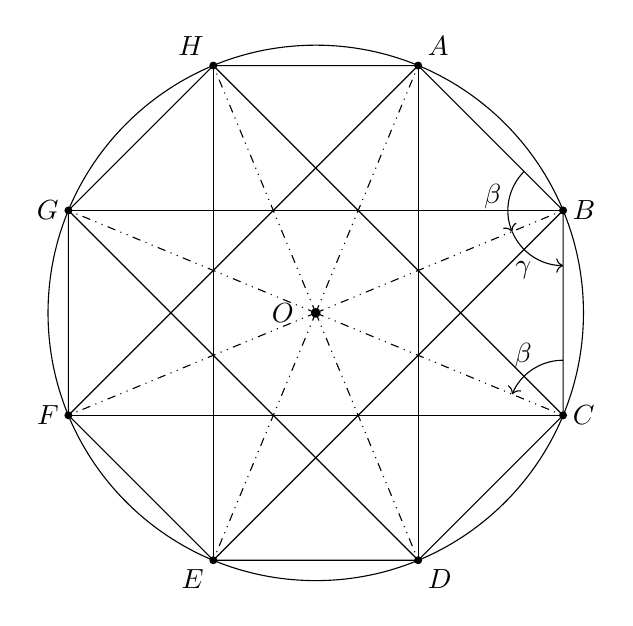
\begin{tikzpicture}[scale=1.7]

	% ---- parameters

	\def\numsides{8}
	\def\radius{2}
	\def\rotation{67.5}

	% ---- coordinates

	\coordinate (O) at (0,0);

	\foreach \i in {1,...,\numsides} {
		\coordinate (P\i) at ({360/\numsides*(\i-1)+\rotation}:\radius);
	}

	% ---- circle

	\draw (O) circle (\radius);

	% ---- polygon

	\draw (P1) \foreach \i in {2,...,\numsides} { -- (P\i) } -- cycle;

	% ---- radiuses

	\foreach \i in {1,...,\numsides} { \draw[dashdotdotted] (O) -- (P\i); }

	% ---- diagonals

	\draw (P1) -- (P4);
	\draw (P4) -- (P7);
	\draw (P7) -- (P2);
	\draw (P2) -- (P5);
	\draw (P5) -- (P8);
	\draw (P8) -- (P3);
	\draw (P3) -- (P6);
	\draw (P6) -- (P1);

	% ---- thick vertices

	\foreach \i in {1,...,\numsides} { \fill (P\i) circle (0.3mm); }

	% ---- vertices labels

	\node[label={[label distance=0.3mm]left:$O$}] at (O) {};
	\filldraw (O) circle (0.9pt);

	\node[above right] at (P1) {$A$};
	\node[right] at (P8) {$B$};
	\node[right] at (P7) {$C$};
	\node[below right] at (P6) {$D$};
	\node[below left] at (P5) {$E$};
	\node[left] at (P4) {$F$};
	\node[left] at (P3) {$G$};
	\node[above left] at (P2) {$H$};

	% ---- angles labels

	\pic[draw, ->, "$\beta$", angle radius=0.7cm, angle eccentricity=1.3]
	{angle = P8--P7--O};

	\pic[draw, ->, "$\gamma$", angle radius=0.7cm, angle eccentricity=1.3]
	{angle = O--P8--P7};

	\pic[draw, ->, "$\beta$", angle radius=0.7cm, angle eccentricity=1.3]
	{angle = P1--P8--O};

\end{tikzpicture}

\end{document}
